\section{\method: Hallucination Detection via Decoupled Representations}
\label{sec:irid}

Building upon the theoretical foundations of HSIC, as introduced in \cref{sec:foundations_hsic}, we propose \method, a single-pass approach for detecting hallucinations in LMs by investigating the internal model representations for input and output. \method~is based on the premise that hallucinations manifest as a quantifiable statistical decoupling between the LM's internal representations of the input sequence and the generated output.
We hypothesize that:
\begin{itemize}
    \item[\textbf{(i)}] \textbf{Sound Generation:} When an LM generates content that is grounded in the input context or in its parametric knowledge, its internal representation of the output, $H_{out}^{(\ell)}$, remains strongly statistically dependent on the internal representation of the input, $H_{in}^{(\ell)}$, at a given layer $\ell$. This strong coupling should result in a substantially positive HSIC value.
    
    \item[\textbf{(ii)}] \textbf{Hallucinated Generation:} Conversely, when an LM hallucinates, the generative process decouples the output representation $H_{out}^{(\ell)}$ from the input representation $H_{in}^{(\ell)}$. As the generated content diverges, these representations become increasingly independent. In such cases, their joint distribution approaches the product of their marginals, leading to an HSIC value close to zero, i.e., $\operatorname{HSIC}(H_{in}^{(\ell)}, H_{out}^{(\ell)}) \approx 0$.
\end{itemize}
\method~leverages this hypothesized drop in HSIC to detect hallucinations. A sufficiently low empirical HSIC score between selected input and output representations suggests a potential hallucination.


\subsection{Problem Formulation}
\label{subsec:irid_problem_formulation}
As defined previously in \cref{sec:background}, $\mathbf{S}_{in} = \{s_1, s_2, \ldots, s_I\}$ is an input token sequence of length $I$, and $\mathbf{S}_{out} = \{t_1, t_2, \ldots, t_O\}$ is the corresponding LM-generated output sequence of length $O$. For a chosen layer $\ell$, the matrix of hidden states for the input sequence is $\mathbf{H}_{in}^{(\ell)} \in \mathbb{R}^{I \times d}$, where $\mathbf{h}_{i,in}^{(\ell)} \in \mathbb{R}^d$ is the hidden state for input token $s_i$, and $d$ is the hidden state dimensionality. Similarly, for the output sequence, $\mathbf{H}_{out}^{(\ell)} \in \mathbb{R}^{O \times d}$, with rows $\mathbf{h}_{j,out}^{(\ell)} \in \mathbb{R}^d$.

To apply HSIC, we define random variables $X$ and $Y$ based on these representations:
\begin{definition}
\label{def:irid_random_variables}
\textit{Let $\mathcal{T}_{in}$ be the set of all possible token types that can be selected from an input sequence, and $\mathcal{T}_{out}$ be the set of all possible token types from an output sequence. We define two random variables, $X$ and $Y$, as :
\begin{itemize}
    \item $X: \mathcal{T}_{in} \to \mathbb{R}^d$, where for any selected input token type $\sigma_{in} \in \mathcal{T}_{in}$ (which, in a specific instance, corresponds to a token $s_i \in \mathbf{S}_{in}$), $X(\sigma_{in}) = \mathbf{h}_{i,in}^{(\ell)}$. The codomain of $X$ is $\mathcal{X} = \mathbb{R}^d$.
    \item $Y: \mathcal{T}_{out} \to \mathbb{R}^d$, where for any selected output token type $\sigma_{out} \in \mathcal{T}_{out}$ (which, in a specific instance, corresponds to a token $t_j \in \mathbf{S}_{out}$), $Y(\sigma_{out}) = \mathbf{h}_{j,out}^{(\ell)}$. The codomain of $Y$ is $\mathcal{Y} = \mathbb{R}^d$.
\end{itemize}}
\textit{For a single input-output pair $(\mathbf{S}_{in}, \mathbf{S}_{out})$, we independently select $n_{\text{eff}}$ tokens from $\mathbf{S}_{in}$ and $\mathbf{S}_{out}$, respectively, to obtain samples $\{x_1, \dots, x_{n_{\text{eff}}}\}$ for $X$ and $\{y_1, \dots, y_{n_{\text{eff}}}\}$ for $Y$. These form the two sets of observations for calculating empirical HSIC.}
\end{definition}


\subsection{\method~Score Computation}
\label{subsec:irid_algorithm_score}
The \method~framework for detecting hallucination in a single generation pass is summarized in Algorithm~\ref{alg:hide}. \changed{By \emph{single-pass}, we mean that \method~requires no additional forward passes of the language model beyond the standard auto-regressive generation of a single output sequence. The keyword extraction step operates on the generated text and uses a lightweight embedding-based ranking model; it does not alter the LM's generation process or require additional decoding steps. Consequently, the dominant computational cost of \method~remains the original generation pass, distinguishing it from multi-pass detection methods that require multiple generations per input.
}

A key component of the proposed method is the computation of our HSIC-based score. The standard unbiased HSIC estimator, $\widehat{\operatorname{HSIC}}_u$ (c.f. Equation~\ref{eq:unbiased_HSIC_foundation}), provides desirable statistical properties but is formally defined for $n \ge 4$ samples. In practical scenarios, particularly when processing short input or output sequences, the effective number of selected tokens, $n_{\text{eff}}$, may fall below this threshold. To ensure the applicability of our framework across all sequence lengths and maintain numerical stability, we employ a pragmatically adapted HSIC-like score, denoted by $\widehat{\operatorname{HSIC}}_{\text{\method}}$. This adaptation modifies the denominators in the standard unbiased HSIC estimator (Equation~\ref{eq:unbiased_HSIC_foundation}) by replacing terms of the form $(n - c)$ with $n$, and substituting the overall scaling factor $1/(n(n - 3))$ with $1/n^2$.

\begin{definition}
\label{def:hsic_irid_modified}
\textit{For an effective sample size $n \ge 1$, the $\widehat{\operatorname{HSIC}}_{\text{\method}}$ score is computed as:}
\begin{multline}
\widehat{\operatorname{HSIC}}_{\text{\method}}(X,Y) = \frac{1}{n^2} \bigg[ 
\text{Tr}(\tilde{\mathbf{K}}_X\tilde{\mathbf{K}}_Y) +
\frac{(\mathbf{1}^T \tilde{\mathbf{K}}_X \mathbf{1}) (\mathbf{1}^T \tilde{\mathbf{K}}_Y \mathbf{1})}{n^2} - \frac{2}{n} \mathbf{1}^T \tilde{\mathbf{K}}_X\tilde{\mathbf{K}}_Y \mathbf{1} \bigg]
\label{eq:hide-score}
\end{multline}
\textit{where $\tilde{\mathbf{K}}_X, \tilde{\mathbf{K}}_Y$ are the $n \times n$ Gram matrices with zeroed diagonals, and $\mathbf{1}$ is an $n \times 1$ vector of ones.}
\end{definition}
While this adaptation introduces bias relative to the standard $\widehat{\operatorname{HSIC}}_u$, it yields a score that is well-defined and numerically stable for any $n \ge 1$. This practical modification allows for consistent application of our method across all encountered data instances. We posit that $\widehat{\operatorname{HSIC}}_{\text{\method}}$ still serves as a valuable and usable heuristic for quantifying the relative strength of dependence, demonstrating its empirical effectiveness in detecting hallucinations in ~\cref{sec:results}.


\begin{algorithm}[ht!]
% \small
%\renewcommand{\thealgorithm}{} 
\caption{\textbf{\method}: Hallucination Detection via Decoupled Representations}
\label{alg:hide}
\begin{algorithmic}[1]
\Statex \textbf{Input:} Input sequence $\mathbf{S}_{in}$, Language model $M$, Layer index $\ell$, Token budget $n_{\text{eff}}$, RBF kernel bandwidth $\gamma$, Threshold $\tau$
\Statex \textbf{Output:} Decision: Hallucination or Non-hallucination

\Procedure{DetectHallucination}{$\mathbf{S}_{in}, M, \ell, n_{\text{eff}}, \gamma, \tau$}
    \State Initialize storage:
        \Statex \hspace{1em} $\mathbf{H}_{\mathrm{in}}^{(\ell)} \leftarrow [\,]$, \quad $\mathbf{H}_{\mathrm{out}}^{(\ell)} \leftarrow [\,]$
    \State Feed input $\mathbf{S}_{in}$ and auto-regressively generate output $\mathbf{S}_{out}$:
    \For{each token $t$ generated by $M$ during inference}
        \State Compute hidden states at layer $\ell$
        \If{$t \in \mathbf{S}_{in}$}
            \State Append its hidden representation to $\mathbf{H}_{\mathrm{in}}^{(\ell)}$
        \Else
            \State Append to $\mathbf{H}_{\mathrm{out}}^{(\ell)}$
        \EndIf
    \EndFor
    \State Now $\mathbf{H}_{\mathrm{in}}^{(\ell)}, \mathbf{H}_{\mathrm{out}}^{(\ell)}$ hold all relevant states

    \State $n_{\text{eff}} \gets \min(n_{\text{eff}}, |\mathbf{S}_{in}|, |\mathbf{S}_{out}|)$
    \If{$n_{\text{eff}} < 1$}
        \State \Return Undetermined
    \EndIf

    \State Identify top-$n_{\text{eff}}$ key-tokens:
        \Statex \hspace{1em} $\mathcal{K}_{\mathrm{in}} \leftarrow \text{KeyBERT}(\mathbf{S}_{\mathrm{in}}, n_{\text{eff}})$
        \Statex \hspace{1em} $\mathcal{K}_{\mathrm{out}} \leftarrow \text{KeyBERT}(\mathbf{S}_{\mathrm{out}}, n_{\text{eff}})$

    \State Collect hidden vectors for selected tokens:
        \Statex \hspace{1em} $\mathbf{X} \leftarrow \{\mathbf{h}_{i,\mathrm{in}}^{(\ell)} \mid \text{token}_i \in \mathcal{K}_{\mathrm{in}}\}$
        \Statex \hspace{1em} $\mathbf{Y} \leftarrow \{\mathbf{h}_{j,\mathrm{out}}^{(\ell)} \mid \text{token}_j \in \mathcal{K}_{\mathrm{out}}\}$

    \State Build RBF kernel $k_{\mathrm{rbf}}$ with bandwidth $\gamma$
    \State Compute HIDE score:
        \Statex \hspace{1em} $\text{score} \gets \widehat{\mathrm{HSIC}}_{\mathrm{HIDE}}(\mathbf{X}, \mathbf{Y}; k_{\mathrm{rbf}})$

    \If{$\text{score} < \tau$}
        \State \Return Hallucination
    \Else
        \State \Return Non-hallucination
    \EndIf
\EndProcedure
\end{algorithmic}
\end{algorithm}

\changed{
\paragraph{Theoretical Properties}
The \method~score inherits several desirable properties from HSIC, including sensitivity to
non-linear dependence and robustness under representation transformations. A formal analysis
of these properties is provided in Appendix A.3.
}

\subsection{Methodological Choices}
\label{subsec:irid_choices}

Our design involves two key choices that must be fixed before the
\method~score can be evaluated:  
(\textit{i}) how to align the \emph{token sets} drawn from the input-output
sequences so that the \emph{same} number of samples are drawn for both random variables $X$ and $Y$, and
(\textit{ii}) from which  \emph{decoder layer}, $\ell\!\in\!\{1,\dots,L\}$ the
hidden-state matrices $\mathbf H^{(\ell)}_{\text{in}}$ and
$\mathbf H^{(\ell)}_{\text{out}}$ are taken.  We formalise the two
choices below and motivate the instantiations that are used throughout the
paper.

\subsubsection{Strategy for Aligning the Sets of Input and Output Samples}
\label{sec:token_alignment}
Let $\mathbf H^{(\ell)}_{\text{in}}\!\in\!\mathbb R^{I\times d}$ and
$\mathbf H^{(\ell)}_{\text{out}}\!\in\!\mathbb R^{O\times d}$ be the matrices
of hidden states for the input and output sequences, respectively, at layer $\ell$, where $I$ and $O$ may differ by in magnitude.  
To guarantee that $X$ and $Y$ are constructed from the \emph{same} effective
sample size, $n_{\text{eff}}$, we consider two principled strategies:

\begin{enumerate}[leftmargin=1.2em,label=(\roman*)]
\item\textbf{Keyword-based Subsampling.}\;
  Let $n_{\text{eff}}$ be our \emph{token budget}, i.e., the number of representative tokens we want to select from both the input and output. Since, in some cases, the input or the output can be smaller than our token budget, we set the value of $n_{\text{eff}}$ to be the minimum of our chosen token budget, input length and output length. We then extract a set of $n_{\text{eff}}$ salient tokens
  $\mathcal K_{\text{in}}\subseteq \mathbf{S}_{\text{in}}$ and
  $\mathcal K_{\text{out}}\subseteq \mathbf{S}_{\text{out}}$ using KeyBERT, which acts as a maximal-marginal-relevance ranker. 
  The aligned sample sets are then
  $\mathcal X=\{\,\mathbf h^{(\ell)}_{i,\text{in}}\mid s_i\!\in\!\mathcal
  K_{\text{in}}^{(n_{\text{eff}})}\}$ and
  $\mathcal Y=\{\,\mathbf h^{(\ell)}_{j,\text{out}}\mid
  t_j\!\in\!\mathcal K_{\text{out}}^{(n_{\text{eff}})}\}$, where the superscript
  $n_{\text{eff}}$ denotes truncation to the top-$n_{\text{eff}}$ representative tokens.  In practice we
  use $n_{\text{eff}}=20$ for our experiments, unless explicitly specified otherwise. We discuss more on the effect of varying our token budget in~\cref{sec:token_budget}. 

\item\textbf{Rank-truncated SVD Alignment.}\;
  Alternatively, we avoid lexical heuristics altogether and enforce equal
  sample size by projecting \emph{both} matrices $\mathbf H^{(\ell)}_{\text{in}}$ and $\mathbf H^{(\ell)}_{\text{out}}$ to subspaces with the same rank (i.e., $n_{\text{eff}})$.
  Concretely, for $\mathbf H^{(\ell)}_{\text{in}}$ we compute a thin SVD
  $\mathbf H^{(\ell)}_{\text{in}}
     =\mathbf U_{X}\,\boldsymbol\Sigma_{X}\mathbf V_{X}^{\top}$ and retain the
  $n_{\text{eff}}$ largest singular directions,
  \begin{equation}
     \mathbf X_{r}
        =\boldsymbol\Sigma_{X}^{(n_{\text{eff}})}\,
         \bigl(\mathbf V_{X}^{(n_{\text{eff}})}\bigr)^{\!\top}\in\mathbb R^{n_{\text{eff}}\times d}.
  \end{equation}
  An analogous projection $\mathbf Y_{r}$ is obtained for
  $\mathbf H^{(\ell)}_{\text{out}}$, yielding aligned sample sets
  $\mathcal X=\{\mathbf x_{r}^{(1)},\dots,\mathbf x_{r}^{(n_{\text{eff}})}\}$ and
  $\mathcal Y=\{\mathbf y_{r}^{(1)},\dots,\mathbf y_{r}^{(n_{\text{eff}})}\}$.
  As both $\mathbf X_{r}$ and $\mathbf Y_{r}$ now contain exactly $n_{\text{eff}}$
  \emph{orthogonal} rows, the empirical Gram matrices in Equation~\eqref{eq:hide-score} have identical dimensions, eliminating the need for any further padding or truncation. We discuss the performances of \method~with both these alignment strategies in~\cref{sec:token_selection}. Unless stated otherwise, we adopt the keyword-based subsampling strategy for our experiments.
\end{enumerate}

\subsubsection{Layer Selection}
Each decoder layer captures different levels of abstraction; therefore, the choice of $\ell$ can, in principle, influence the measured dependence. Based on prior work suggesting that representations corresponding to the middle layers are often richer \citep{skean2025layerlayeruncoveringhidden} and provide stronger sentence-level semantic information suitable for detecting inconsistencies \citep{azaria2023internalstatellmknows}, we fix $\ell=\ell_{\text{mid}}$ for all our experiments to avoid an additional hyperparameter sweep. However, our framework is flexible to any layer choice and we observe the performance of \method~to be almost agnostic to the choice of $\ell$ (\cref{sec:layer_choice}).


\subsection{Structural Validation of Decoupling}
\label{sec:structural_validation}
\changedtwo{
While HIDE provides a statistical measure of input-output dependence, we seek to ground this decoupling in the internal operations of the autoregressive transformer. Specifically, we investigate how reductions in the HSIC score correlate with bottlenecks in the attention-mediated information flow to the residual stream, and how this dynamic differentiates faithfulness from factuality hallucinations.
}
\changedtwo{
As defined in \cref{sec:background}, $\mathbf{S}_{in} = \{s_1, s_2, \ldots, s_I\}$ is the input prompt and $\mathbf{S}_{out} = \{t_1, t_2, \ldots, t_O\}$ is the generated output sequence.
In a standard transformer decoder, the hidden state of the $j$-th generated token at layer $l$, denoted $h_{j,out}^{(l)} \in \mathbb{R}^d$, is constructed via successive updates to the residual stream:
$$h_{j,out}^{(l)} = h_{j,out}^{(l-1)} + \text{MHA}(h_{j,out}^{(l-1)}, H_{ctx}^{(l-1)}) + \text{MLP}(\tilde{h}_{j,out}^{(l)})$$
where $H_{ctx}^{(l-1)}$ represents the concatenated context of the input and preceding output tokens. The Multi-Head Attention (MHA) mechanism projects information from the context into the current token's representation across $H$ heads. The contextual update $A_j$ written to the residual stream is bounded by the convex combination of value vectors:
$$A_j = \sum_{h=1}^H W_O^{(h)} \left( \sum_{i=1}^I \alpha_{j,i}^{(h)} W_V^{(h)} h_{i,in}^{(l-1)} + \sum_{k=1}^j \beta_{j,k}^{(h)} W_V^{(h)} h_{k,out}^{(l-1)} \right)$$
where $W_O^{(h)}$ and $W_V^{(h)}$ are the output and value projection matrices, and $\alpha_{j,i}^{(h)}$ and $\beta_{j,k}^{(h)}$ are the softmax attention weights.
}

\changedtwo{
To trace this flow at our target layer ($l=l_{mid}$), we extract two structural proxies. The first is the \textit{Attention Mass to Prompt} ($\Omega$), representing the aggregate cross-attention probability mass directed from the generated output tokens back to the input prompt context. For a given token $j$, this is defined as $\Omega_j = \frac{1}{H} \sum_{h=1}^H \sum_{i=1}^I \alpha_{j,i}^{(h)}$. The second proxy is the \textit{Input-Derived Update Norm} ($\Delta_{in}$), which measures the $L_2$ norm of the specific residual stream vector updates originating exclusively from the input tokens. This is formally defined as $\Delta_{j,in} = ||\sum_{h=1}^H W_O^{(h)} \sum_{i=1}^I \alpha_{j,i}^{(h)} W_V^{(h)} h_{i,in}^{(l-1)}||_2$, and approximated in our experiments as the magnitude of the raw cross-attention probabilities multiplied by the preceding layer's hidden states.
}

\changedtwo{
A critical consideration is whether a single dependence-based lens can capture both faithfulness and factuality errors. We postulate that while the underlying failure modes differ, both are strongly associated with structural decoupling in the residual stream. In faithfulness tasks, accurate generation requires explicit routing from the source evidence ($\Omega \gg 0$). When the model hallucinates, it frequently bypasses the input context ($\Omega \to 0$) to rely on internal priors or local decoding history. Consequently, the output representation becomes substantially less dependent on the input, leading the joint probability distribution to factorize ($P_{XY} \approx P_X P_Y$). Conversely, factuality hallucinations for closed-book queries represent a parametric failure. Faithful factual recall requires strong attention to specific subject-relation tokens to trigger correct associative memories in the MLP sub-layers. If this knowledge is absent, the specific structural circuit weakens, reducing the mutual information $I(X;Y)$. In both scenarios, the structural breakdown corresponds to a shrinking of the cross-covariance operator $C_{XY}$, which directly yields a reduced HIDE score.
}

\changedtwo{
As illustrated in Figure \ref{fig:structural_flow}, empirical evaluation validates this explanatory framework. The HIDE score exhibits a strong positive correlation with $\Omega$ across both Llama-3-8B and Gemma-2-9B on faithfulness (SQuAD) and factuality (Natural Questions) benchmarks (e.g., Pearson Correlation Coefficient $PCC=0.749$ and $0.805$ for Llama-3-8B). When generations are faithful, the model anchors its attention to the input. During hallucinations, the model bypasses the input, causing the HIDE score to collapse. Conversely, we observe a weak or negative correlation between the HIDE score and the update norm $\Delta_{in}$ (e.g., $PCC=-0.207$ for Llama-3-8B on SQuAD). This highlights a critical magnitude versus precision dynamic: massive residual updates do not guarantee faithful information transfer. During a hallucination, the model often pulls a noisy, unrefined amalgamation of states into the residual stream, inflating $\Delta_{in}$ without preserving semantic alignment. By capturing non-linear dependencies via HSIC, HIDE successfully isolates genuine statistical alignment from mere vector magnitude.
}

{\paragraph{Differentiating Faithfulness and Factuality} 
\changedtwo{To verify that HIDE isolates causal operations rather than merely exploiting dataset regularities (such as detecting strictly off-topic text), we evaluated the Question-Conditioned but Wrong (QCBW) subset within the Natural Questions dataset. This subset comprises factuality hallucinations that maintain high semantic similarity (top 25\%) to the input prompt. As shown in Figure \ref{fig:structural_flow} (indicated by star markers), QCBW instances heavily cluster in the low-HIDE, low-$\Omega$ region. Even if the output remains superficially on-topic, the failure of precise associative mapping forces the model to default to diffuse, high-entropy priors, confirming that representational decoupling accurately captures the underlying structural collapse across both failure modes.
}

\begin{figure*}[t]
    \centering
    \begin{subfigure}[b]{0.49\textwidth}
        \centering
        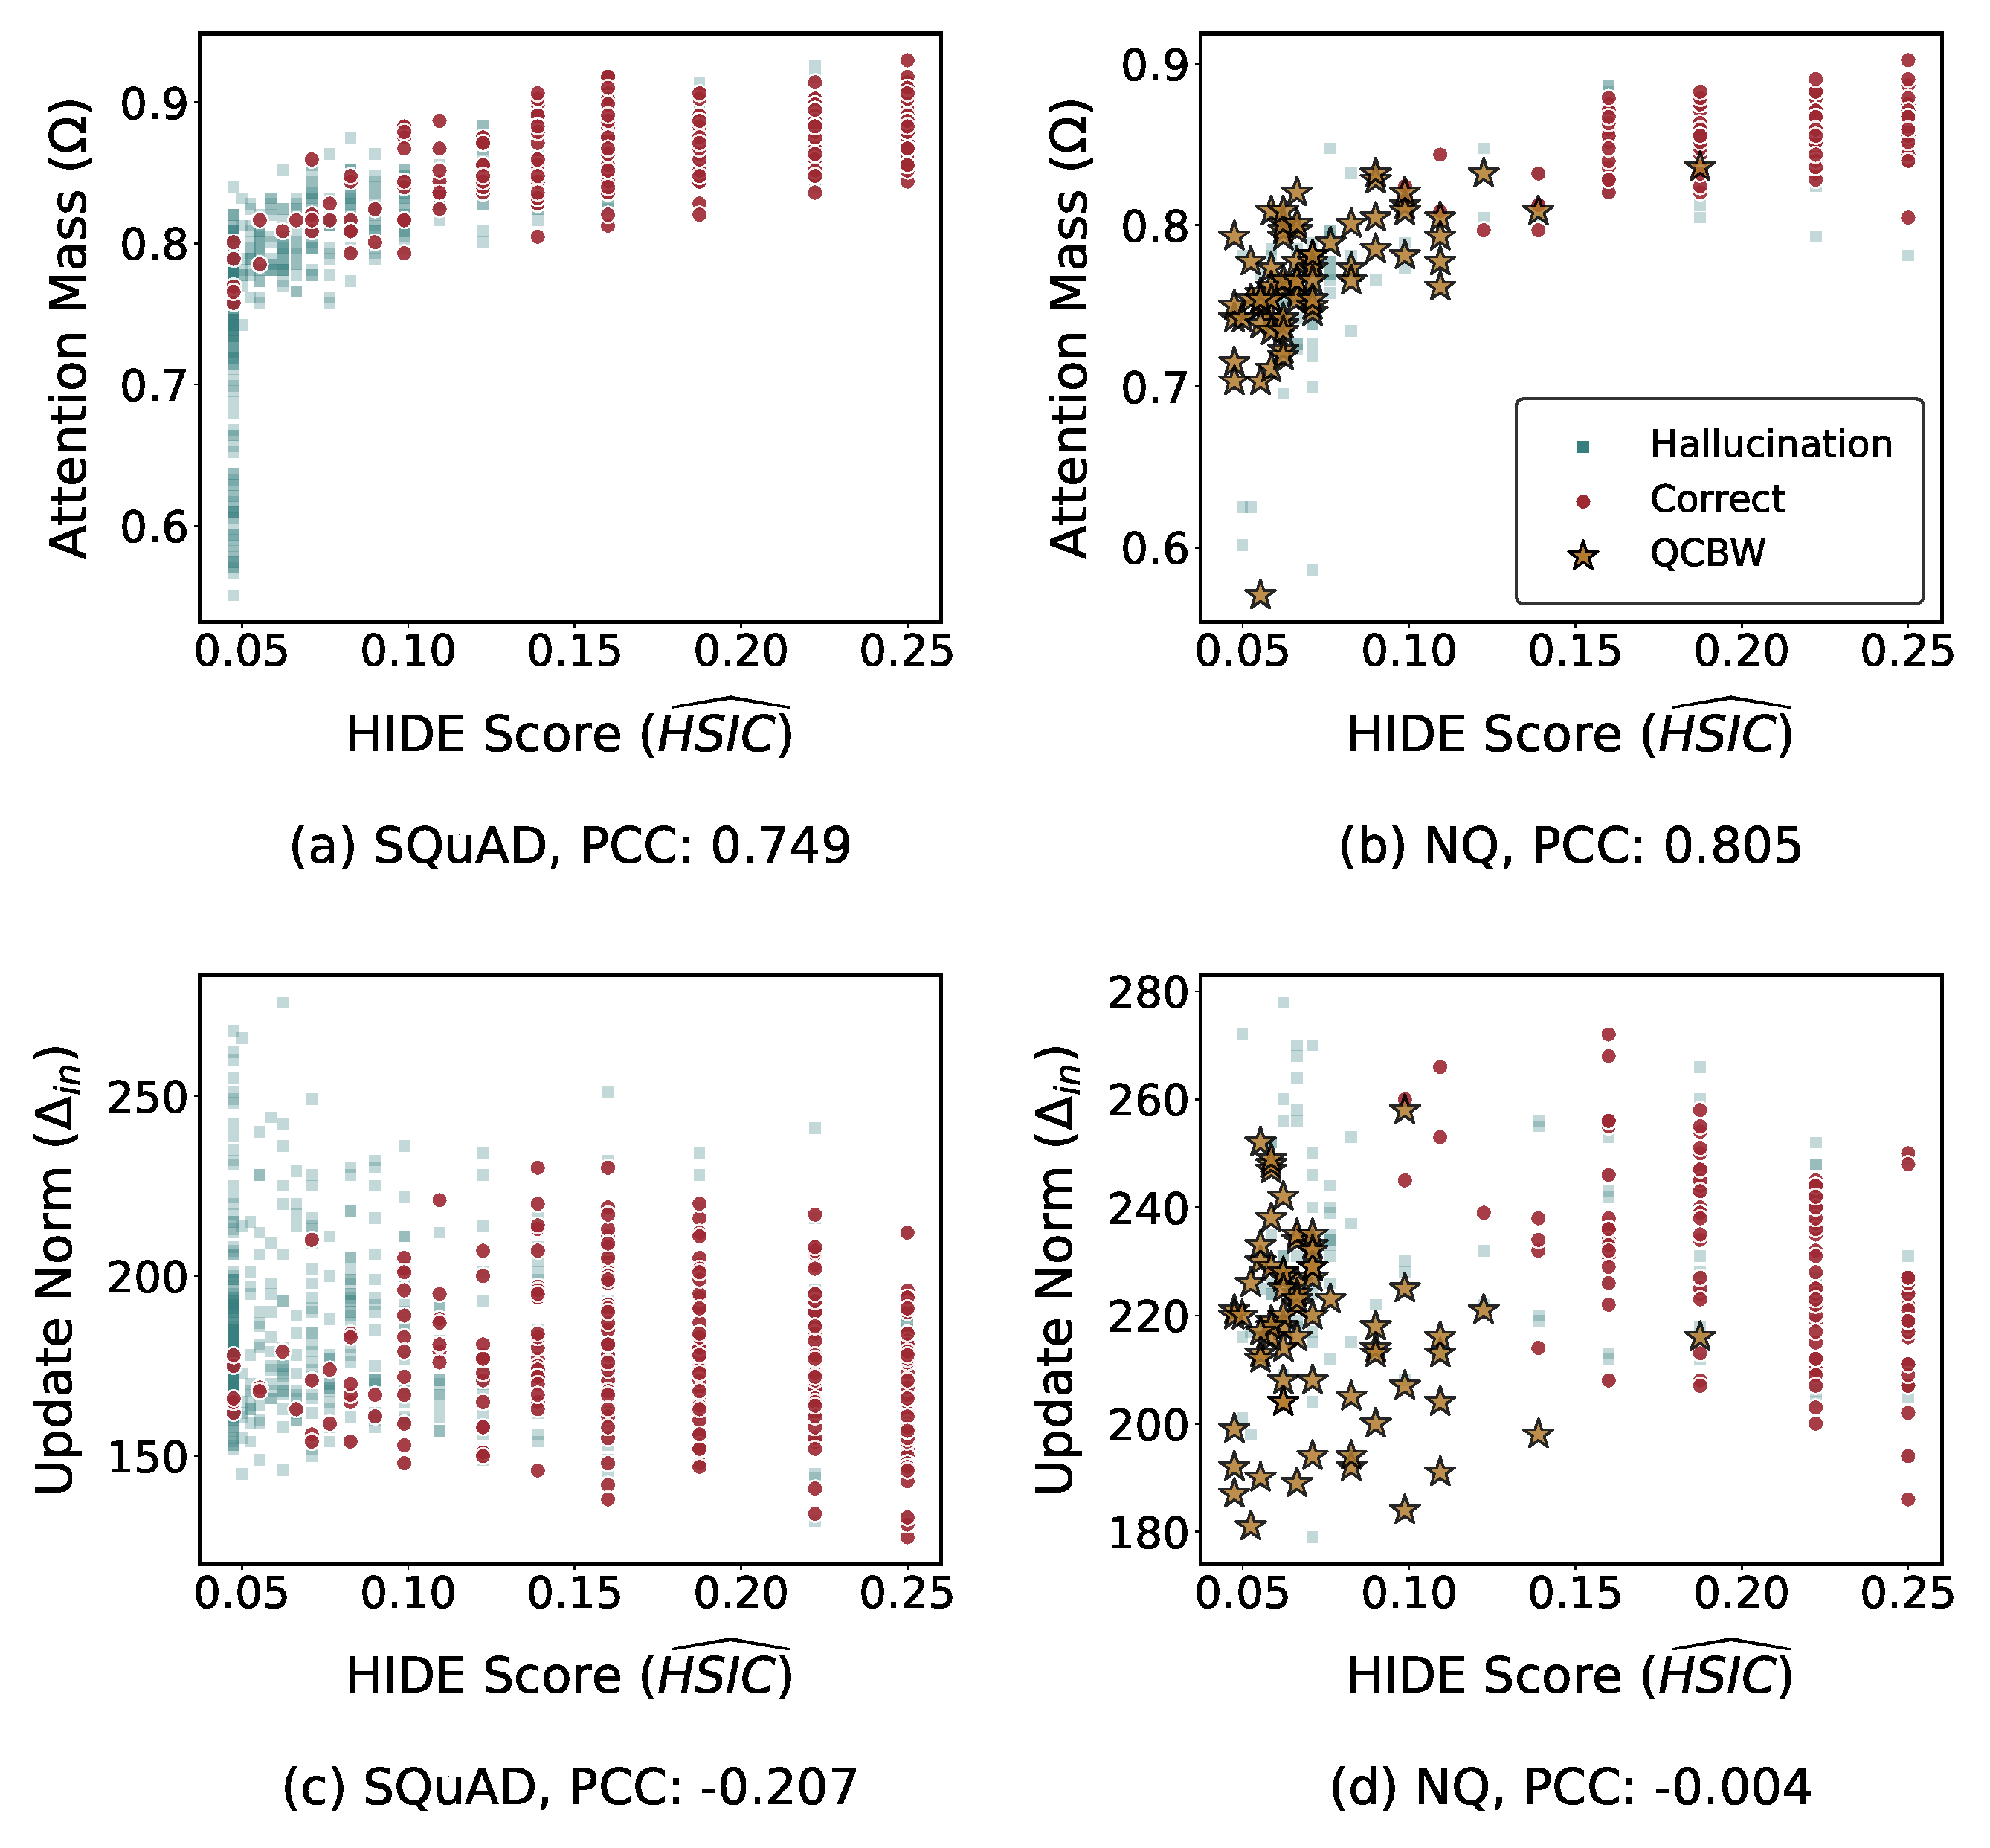
\includegraphics[width=\textwidth]{files/figures/llama3-8b_Mechanistic_Flow.pdf}
        \caption*{(i) Llama-3-8B}
    \end{subfigure}
    \hfill
    \begin{subfigure}[b]{0.49\textwidth}
        \centering
        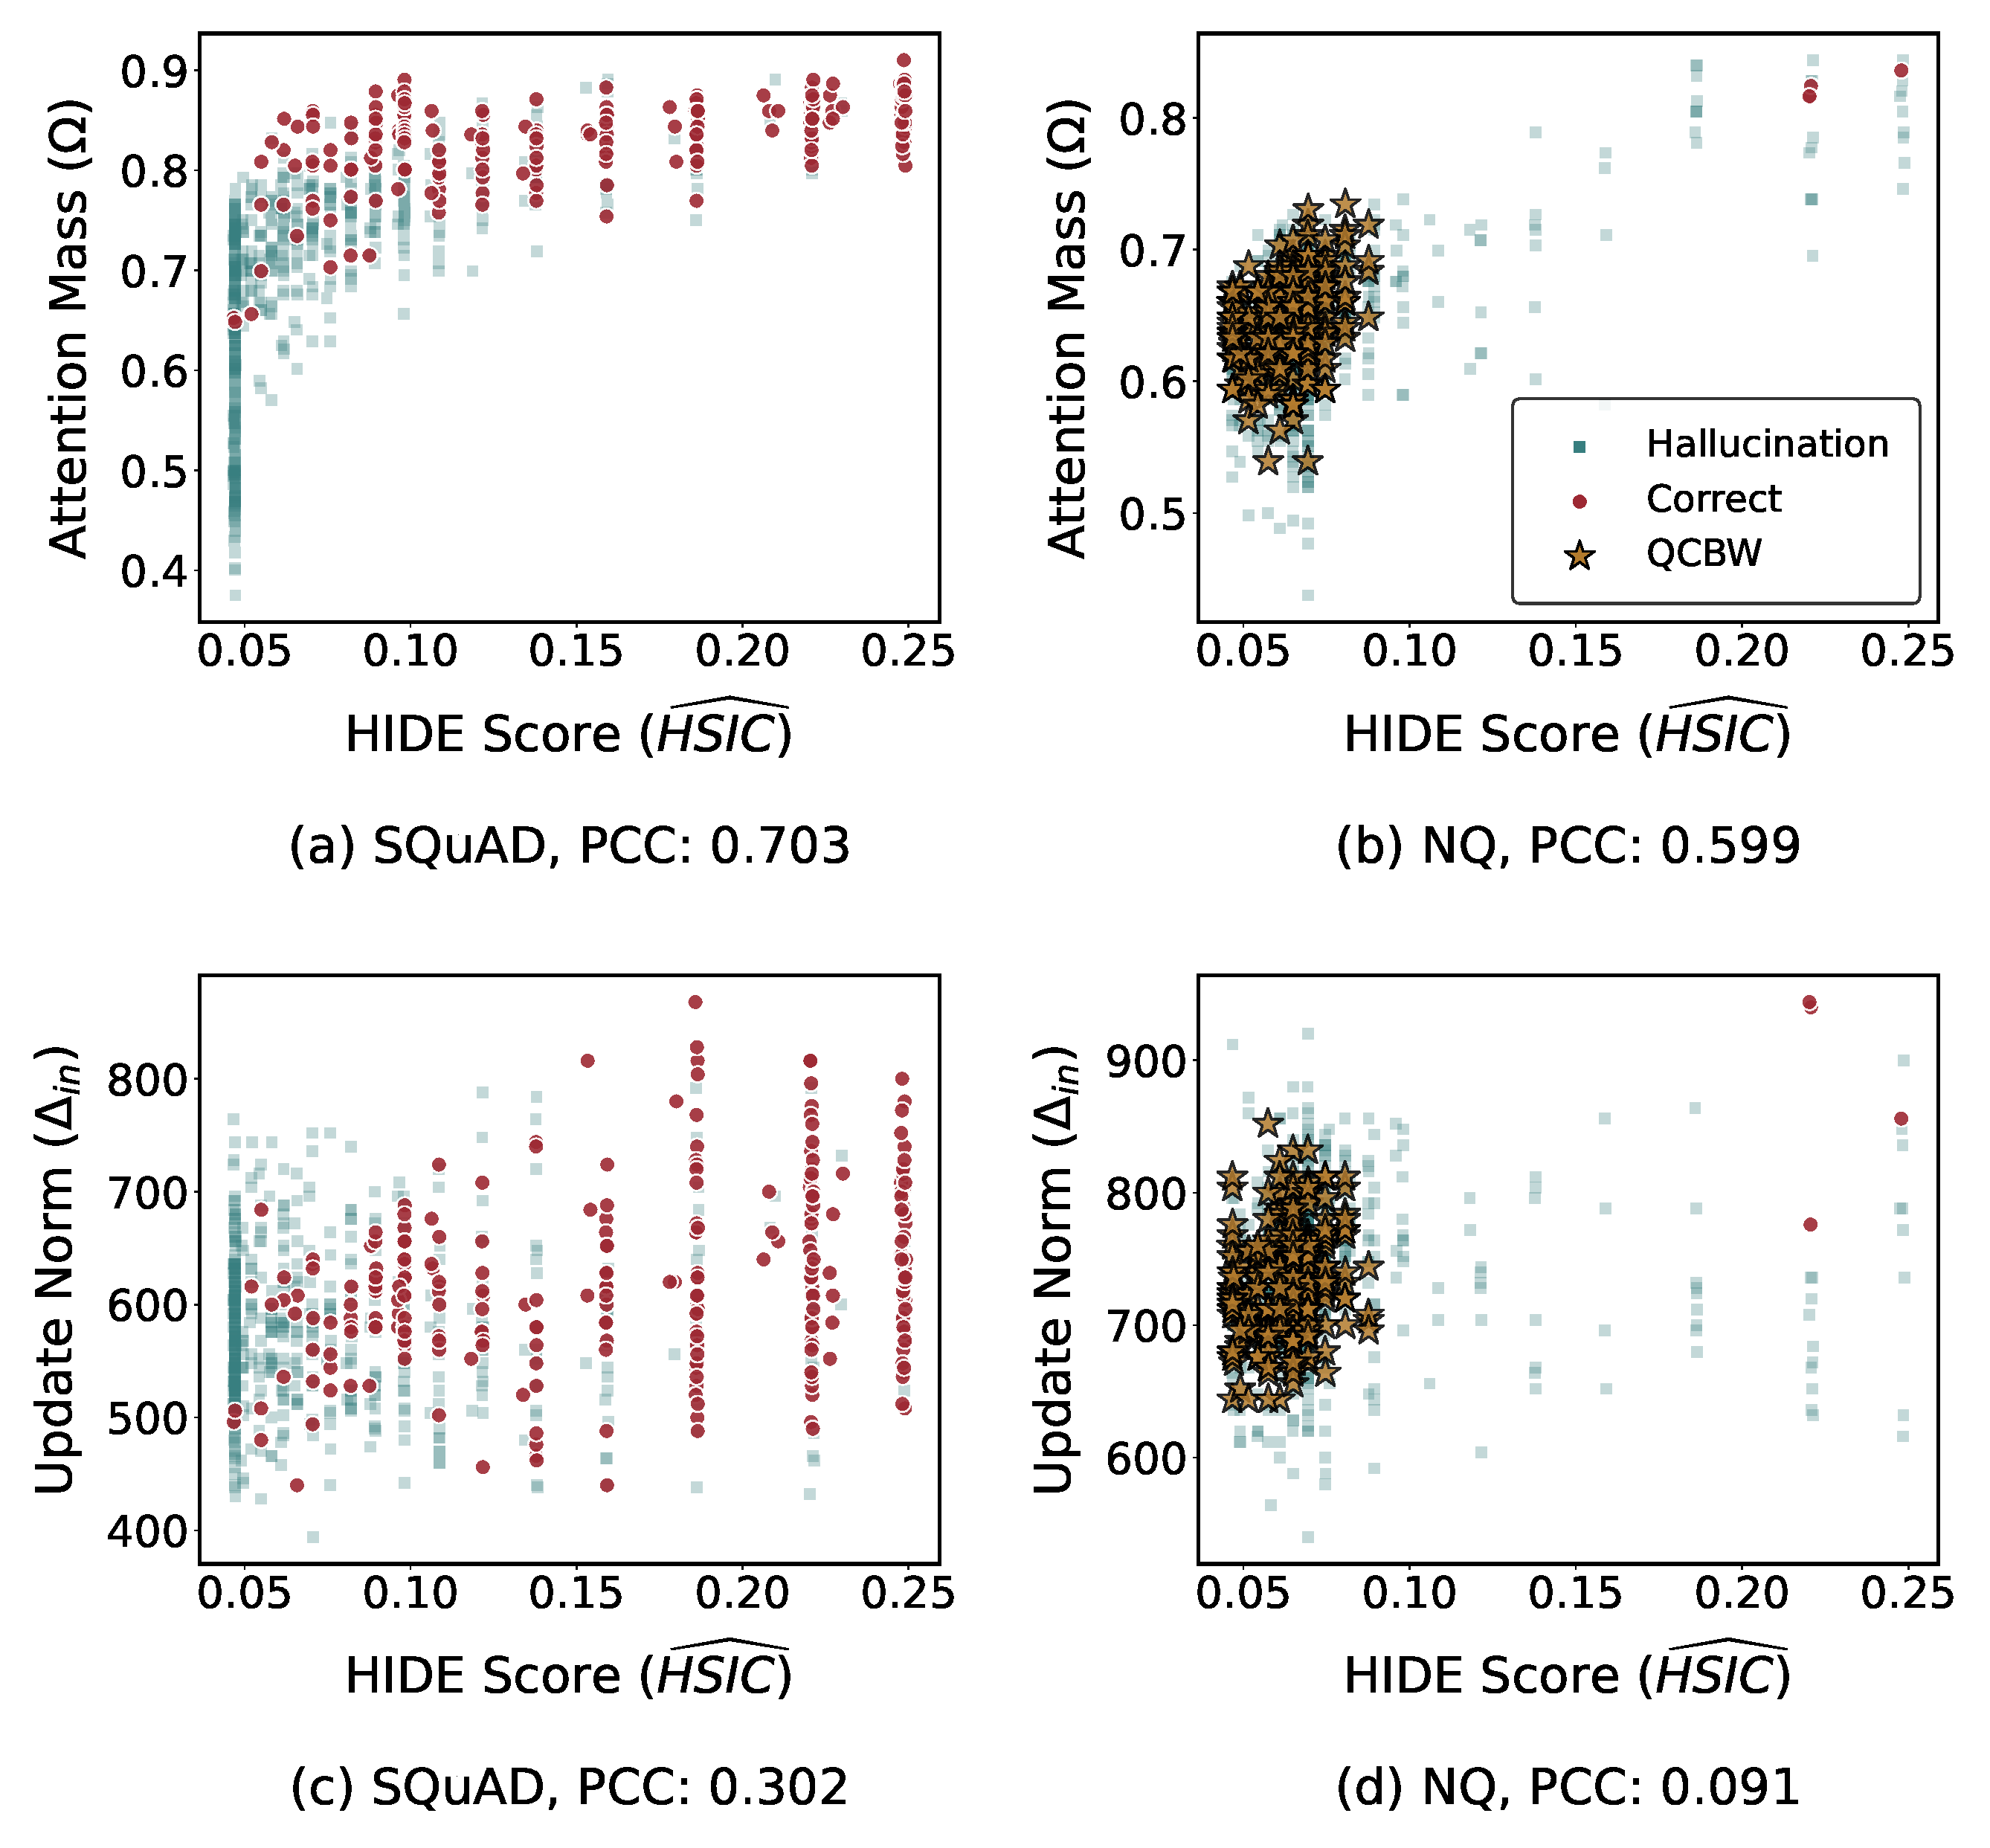
\includegraphics[width=\textwidth]{files/figures/gemma-2-9b_Mechanistic_Flow.pdf}
        \caption*{(ii) Gemma-2-9B}
    \end{subfigure}
    \caption{\changedtwo{Internal flow analysis of Llama-3-8B and Gemma-2-9B. The HIDE score strongly correlates with Attention Mass ($\Omega$) but shows weak/negative correlation with the Update Norm ($\Delta_{in}$), illustrating the magnitude vs. precision dynamic. QCBW hallucinations (star markers) demonstrate structural decoupling even when semantically on-topic.}}
    \label{fig:structural_flow}
\end{figure*}
